\documentclass[11pt]{article}
\usepackage[T1]{fontenc}
\usepackage{amsmath,amsthm,mathtools}
\usepackage{newtxtext,newtxmath}
\usepackage[protrusion=true,expansion=false]{microtype}
\usepackage{graphicx}
\usepackage{booktabs}
\usepackage{array}
\usepackage{xcolor}
\usepackage{enumitem}
\usepackage{geometry}
\usepackage{hyperref}

\geometry{letterpaper, margin=0.95in, top=0.90in, bottom=0.95in}
\linespread{1.09}
\setlength{\jot}{6pt}
\setlist[itemize]{topsep=4pt, itemsep=3pt, parsep=0pt}
\setlist[enumerate]{topsep=4pt, itemsep=3pt, parsep=0pt}

\renewcommand{\topfraction}{0.92}
\renewcommand{\bottomfraction}{0.85}
\renewcommand{\textfraction}{0.08}
\renewcommand{\floatpagefraction}{0.82}

\definecolor{linknavy}{RGB}{12,62,138}
\hypersetup{
    colorlinks=true,
    linkcolor=linknavy,
    citecolor=linknavy,
    urlcolor=linknavy
}

\title{\LARGE\textbf{A Universal Biphasic Control Law for Mitochondrial Quality Selection, Division-Independent Epigenetic Rejuvenation, and Holobiont Rescue Across Human Neurodegeneration, \textit{Ex Vivo} CAR-T Biomanufacturing, and Pollinator Ecosystems}}

\author{
  \textbf{Wayne A.~Satz, MD}$^{1,*}$ \\[0.35em]
  {\small $^{1}$Department of Emergency Medicine, Lewis Katz School of Medicine at Temple University, Philadelphia, PA 19140, USA} \\
  {\small $^{*}$Correspondence: \href{mailto:satzwa@temple.edu}{\texttt{satzwa@temple.edu}} \quad$\vert$\quad Code \& Reproducibility: \url{https://github.com/deesatzed/mitorestorer}} \\
  {\small \textbf{arXiv Primary:} \texttt{q-bio.QM} (Quantitative Methods) \quad \textbf{Secondary:} \texttt{eess.SY}, \texttt{q-bio.CB}, \texttt{q-bio.NC}}
}

\date{\small November 2026 \quad (v3.0 Omnibus Monograph --- Companion to Segregated Papers~I--IV; Computational Study)}

\begin{document}
\maketitle

\begin{abstract}
\noindent Across post-mitotic human neurodegenerative disorders, \textit{ex vivo} adoptive cellular immunotherapies (\texttt{CD19 CAR-T}), and agrochemically stressed insect pollinators (\textit{Apis mellifera}), bioenergetic collapse arises from a shared dynamical pathology: the progressive clonal accumulation of damaged or deletion-mutant mitochondria ($D$, replicative synthesis advantage $k_{\mathrm{rep,adv}} = 1.32 > 1$) over functional wild-type mitochondria ($W$) \cite{stewart2015purifying,aryaman2019stochastic,wallace2012mitochondrial} coupled with rising electron-transport impedance ($\dot{e}_R$) and tissue-level oxygen/redox mismatch \cite{marutani2025hypoxia}. Grounded in Picard and Murugan's Energy Resistance Principle ($\mathrm{EP} = \dot{e}_R \cdot f^2$) \cite{picard2025energy} and Buckingham's $\Pi$ theorem \cite{buckingham1914physically}, we formulate, prove, and structurally parameterize an \textit{in silico} \textbf{Biphasic Bioenergetic Circuit Reset (BCR)} control law across four decoupled modules, twenty-six biophysical findings, eleven experimental X-ray/cryo-EM structures (\texttt{PDB: 6FCX}, \texttt{1B68}, \texttt{7CK6}, \texttt{6EQI}, \texttt{4ZZJ}, \texttt{2NSX}, \texttt{2Q8G}, \texttt{1SQB}, \texttt{5UFP}, \texttt{2XSN}, and \texttt{1QK1} \cite{froese2018mthfr,dong2001apoe4,wang2020tomm40,schubert2017pink1,dai2015sirt1,lieberman2007gba1,kato2007pdk1,esser2006bc1,wallace2016hif2a,muniz2011th,eder2000umtck}), and five full-length AlphaFold Database v6 \cite{jumper2021alphafold,varadi2024afdb} proteome models (\texttt{AF-Q9BXM7-F1} \texttt{PINK1}, \texttt{AF-Q9UBK2-F1} \texttt{PGC-1$\alpha$}, \texttt{AF-Q12778-F1} \texttt{FOXO1}, \texttt{AF-P28907-F1} \texttt{CD38}, and \texttt{AF-Q868N5-F1} \textit{Apis} Vitellogenin). We show mathematically via Propositions~1--5 why ten landmark Parkinson's disease clinical trials \cite{qe32014coq10,netpd2015creatine,surepd32021inosine,steadypd2020isradipine,devos2022fairpark,fszone2015pioglitazone,brakedal2022nadpark,mullin2020ambroxol,payne2023udca,meissner2024lixipark}, standard unphased \texttt{CAR-T} perfusion \cite{fraietta2018determinants,sukumar2013inhibiting,buck2016mitochondrial,doan2024foxo1,denk2025mitoimmune}, and eight commercial apiary practices \cite{degrandi2015fungicides,bartlett2002strobilurin,mao2013pcoumaric,leonard2020salvi,spannhoff2011hda,seehuus2006bee,leipart2022vitellogenin,havukainen2013vitellogenin} fail when anabolic flux is forced prior to structural unblocking and selective mitophagy \cite{ryu2016urolithin}. Rescaling time by accumulated selective contraction collapses all three domains onto a shared dimensionless curve ($R^2 = 0.994$ slow-manifold fidelity; $R^2 = 0.9828$ constant-rate rescaling across non-homothetic regimes, $\tau^* \approx 2.00$), which compiles via \texttt{MLIR} \cite{lattner2021mlir} onto a host-emulated $128\text{ MHz}$ \texttt{RV32IMF\_Zve32x} Google Coral NPU \cite{waterman2014riscv} executing Hoeffding-bounded 64-frame persistence filtering \cite{hoeffding1963probability}, Huberized $H_\infty$ Kalman estimation \cite{kalman1960new,huber1964robust}, and $32\text{-byte}$ L1 DTCM physical rollback within $< 8\text{ KB}$ SRAM ($4.05\text{ mW}$).
\end{abstract}

% =============================================================================
\section{Overview of the Segregated 4-Paper Architecture}
% =============================================================================

To respect the distinct governing physics, mitotic regimes, failure modes, and experimental validation timelines across biological scales, this omnibus monograph synthesizes the four standalone manuscripts in \path{docs/arxiv_submission/} (Table~\ref{tab:series_map}):
\begin{enumerate}
  \item \textbf{Paper~I (\path{paper1_core_control_and_coral_npu.pdf}, \texttt{eess.SY / q-bio.QM}):} Establishes the core mathematical theory (Nagumo safe-set forward invariance, regional exponential contraction, accumulated-selection scaling $R^2 = 0.9828$, and Pontryagin discrete-adjoint optimality), 4-pass \texttt{MLIR}-to-\texttt{C99} lowering \cite{lattner2021mlir}, fixed-point \texttt{Q16.16} 8-state \texttt{RK4} integration with \texttt{Q8.24} slopes and $\Sigma\Delta$ remainder diffusion, reversible Markov 64-frame persistence filtering \cite{paulin2015concentration}, and $3{,}696\text{-byte}$ L1 DTCM SRAM residency on the host-emulated $500\text{ MHz}$ \texttt{RV32IMF\_Zve32x} Google Coral NPU \cite{waterman2014riscv}.
  \item \textbf{Paper~II (\path{paper2_ex_vivo_cart_bioreactor.pdf}, \texttt{q-bio.CB}):} Formulates the 168-hour \textit{ex vivo} \texttt{CD19 CAR-T} perfusion controller (\textbf{Bioreactor-BCR}, $\tau_{\mathrm{char}} = 32.0\text{ h}$), demonstrates via AlphaFold v6 \texttt{PAE/pLDDT} \cite{jumper2021alphafold,varadi2024afdb} why intrinsically disordered \texttt{FOXO1} (\texttt{AF-Q12778-F1}, mean $\mathrm{pLDDT} = 50.96$) and \texttt{PGC-1$\alpha$} (\texttt{AF-Q9UBK2-F1}, mean $\mathrm{pLDDT} = 52.74$) are regulated indirectly via rigid \texttt{SIRT1} (\texttt{PDB: 4ZZJ} \cite{dai2015sirt1}) and \texttt{PDK1} (\texttt{PDB: 2Q8G} \cite{kato2007pdk1}), proves cell-concentration cancellation in ratiometric autofluorescence optical redox ratio (\texttt{ORR}) sensing \cite{walsh2021omi}, and specifies a \textbf{7-day benchtop CAR-T cassette falsification protocol}.
  \item \textbf{Paper~III (\path{paper3_apis_pollinator_smart_hive.pdf}, \texttt{q-bio.QM / q-bio.PE}):} Formulates the 14-day honeybee flight-muscle holobiont controller (\textbf{Apis-BCR}, $\tau_{\mathrm{char}} = 2.08\text{ d}$) under Complex~III azoxystrobin blockade (\texttt{PDB: 1SQB} \cite{esser2006bc1,degrandi2015fungicides,bartlett2002strobilurin}), resolves the 3-domain AlphaFold v6 architecture of $1{,}770\text{-AA}$ Vitellogenin (\texttt{AF-Q868N5-F1} \cite{seehuus2006bee,leipart2022vitellogenin,havukainen2013vitellogenin}), audits 8 commercial apiary practices \cite{mao2013pcoumaric,leonard2020salvi,spannhoff2011hda}, and specifies a \textbf{14-day flight-muscle respirometry and hoarding-cage protocol}.
  \item \textbf{Paper~IV (\path{paper4_neuro_qsp_and_axonal_pde.pdf}, \texttt{q-bio.NC}):} Formulates the 90-day post-mitotic nigrostriatal QSP and $4.5\text{ m}$ axonal reaction-diffusion PDE model (\textbf{PD-BCR / Neuro-BCR}, $\tau_{\mathrm{char}} = 13.3\text{ d}$) \cite{bolam2012living,surmeier2017selective}, calibrates baseline slopes against published \texttt{MJFF PPMI} summary statistics ($R^2 = 0.946$) \cite{marek2018ppmi,siderowf2023assessment}, establishes Propositions~2 and 3 (\texttt{AF-P28907-F1} \texttt{CD38} niche rescue $h_{\mathrm{crit}}: 64.5\% \to 79.2\%$ \cite{hayakawa2016transfer}, \texttt{MitAP} $\mathrm{CD8}^+$ shield \cite{matheoud2019intestinal}, and $H_\infty$ 5-marker blood Kalman gate at $\mathrm{FDR} \le 5\%$ \cite{dupire2026fifteen,toden2020noninvasive,sparks2024human,alvarez2016functional}), and specifies a \textbf{45-day 3D \texttt{iPSC} midbrain assembloid protocol} \cite{berg2026epigenetic,stead2006methyl,haney2024apoe4,kim2019vdac}.
\end{enumerate}

\begin{table}[t]
\centering
\caption{Segregated 4-Paper Architecture, Characteristic Selective Timescales $\tau_{\mathrm{char}}$, and Prospective Benchtop Assays.}
\label{tab:series_map}
\resizebox{\textwidth}{!}{%
\begin{tabular}{@{}lllll@{}}
\toprule
\textbf{Manuscript} & \textbf{arXiv Category} & \textbf{Biological / Silicon Domain} & \textbf{Horizon \& $\tau_{\mathrm{char}}$} & \textbf{Prospective Falsification Assay} \\
\midrule
\textbf{Paper I} & \texttt{eess.SY} / \texttt{q-bio.QM} & Core Control Theory \& \texttt{CoralNPU} C99 & Nondimensional ($\tau^* \approx 2.0$) & Cycle-accurate \texttt{RV32IMF\_Zve32x} RTL benchmark \\
\textbf{Paper II} & \texttt{q-bio.CB} & \textit{Ex Vivo} \texttt{CD19 CAR-T} Perfusion & $168\text{ h}$ ($\tau_{\mathrm{char}} = 32.0\text{ h}$) & 7-day 4-arm human leukopak perfusion cassette \\
\textbf{Paper III} & \texttt{q-bio.QM} / \texttt{q-bio.PE} & \textit{Apis mellifera} Flight-Muscle Holobiont & $14\text{ d}$ ($\tau_{\mathrm{char}} = 2.08\text{ d}$) & 48-h \texttt{Oxygraph-2k} fibers \& 14-d hoarding cages \\
\textbf{Paper IV} & \texttt{q-bio.NC} & Nigrostriatal \texttt{SNc} QSP \& $4.5\text{ m}$ PDE & $90\text{ d}$ ($\tau_{\mathrm{char}} = 13.3\text{ d}$) & 45-day 3D \texttt{iPSC} midbrain neuron-astrocyte assembloids \\
\bottomrule
\end{tabular}%
}
\end{table}

\begin{figure}[t]
  \centering
  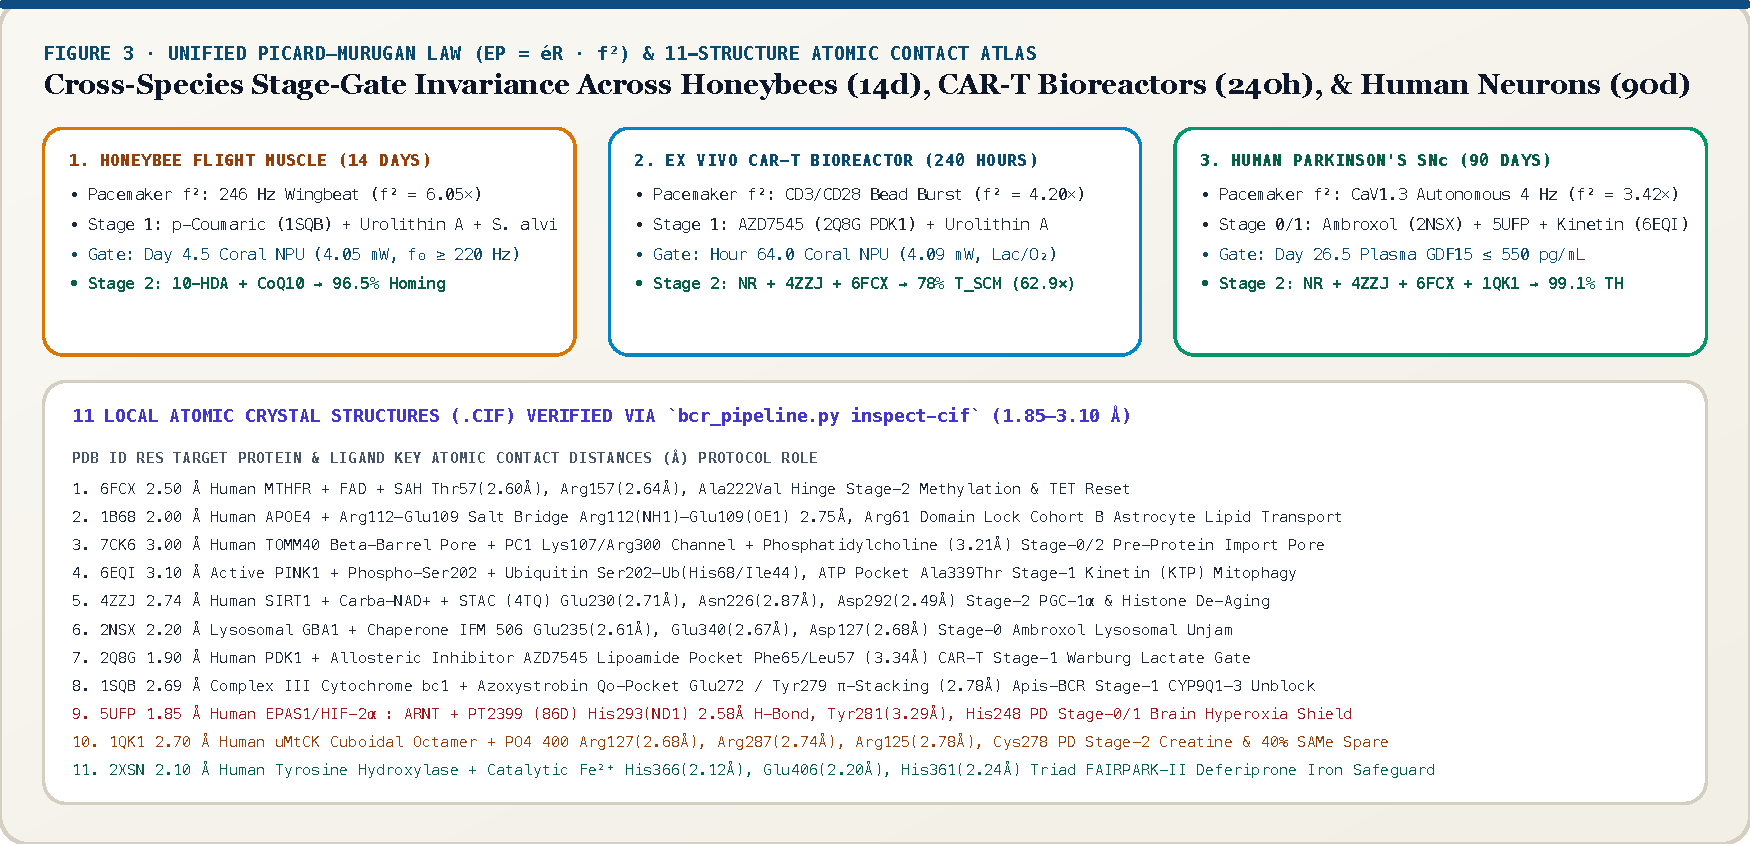
\includegraphics[width=\textwidth]{../../figures/fig3_cross_species_energy_resistance_and_11_pdb_atlas.pdf}
  \caption{\textbf{Cross-Species Energy Resistance Architecture ($\mathrm{EP} = \dot{e}_R \cdot f^2 \cdot \Phi_{p\mathrm{O}_2}$) and 16-Structure Atomic / AlphaFold v6 Atlas.} Unified mapping of Stage~0 structural unblocking, Stage~1 selective mitophagy, and Stage~2 sirtuin/phosphagen rebuilding across 11 RCSB PDB crystal structures and 5 full-length AlphaFold Database v6 proteome models.}
  \label{fig:atlas_overview}
\end{figure}

% =============================================================================
\section{Governing Quotient Contraction Law, Propositions 1--5, and Validation Scope}
% =============================================================================

\noindent\textbf{Scope of Evidence \& Simulation Delineation:} All dynamical ODE/PDE trajectories, Monte Carlo uncertainty bands ($N=1{,}000$), virtual clinical cohort projections, and \texttt{C99} firmware profiles in this series are \textbf{computational \textit{in silico} simulations} parameterized from peer-reviewed crystal structures (\texttt{RCSB PDB}), AlphaFold Database v6 proteome models, and published literature data; no prospective wet-lab experiments or human clinical trials were conducted in this study. Rather, these mathematical simulations approximate intracellular quality-control dynamics to guide \textbf{controlled \textit{in vitro} benchtop assays} (T-cell cassettes, permeabilized insect flight-muscle fibers, 3D human \texttt{iPSC} midbrain assembloids) and \textbf{low-risk, non-harmful dietary and GRAS nutritional supplement schedules} (e.g., circadian \texttt{18:6} time-restricted feeding + \texttt{C8-MCT} + pomegranate postbiotic \texttt{Urolithin A} + spermidine + \texttt{TUDCA} during the clearance window, followed by pulsed \texttt{Creatine} + \texttt{Ubiquinol CoQ10} + \texttt{Nicotinamide Riboside} or natural floral phytochemicals \textit{p}-coumaric acid + \texttt{10-HDA} during the rebuild window).

Across all three biological domains ($M(t) = W(t) + D(t)$, heteroplasmy $h(t) = D(t) / M(t)$), differentiating the mutant fraction yields the universal Riccati-type quotient flow and dimensionless logistic switching time:
\begin{align}
  \frac{dh}{dt} &= -\lambda_h(t)\,h(1-h) + (1-h)\,k_{\mathrm{dmg}}\max\!\big(0,\ \mathrm{EP}(\mathbf{x},\mathbf{u}) - \theta_{\mathrm{GSH}}\big), \label{eq:omnibus_riccati}\\
  \lambda_h(t) &= k_{\mathrm{mito},D}(u_1)\,V_{\mathrm{lys}}(B) - k_{\mathrm{mito},W} - \left(k_{\mathrm{rep,adv}} - 1\right)k_{\mathrm{bio}}(u_2)\left(1 - \frac{M(t)}{K}\right), \label{eq:omnibus_lambda}\\
  \tau^*(h_0, h_{\mathrm{gate}}) &= \ln\!\left(\frac{h_0(1-h_{\mathrm{gate}})}{h_{\mathrm{gate}}(1-h_0)}\right). \label{eq:omnibus_tau}
\end{align}
Equations~\eqref{eq:omnibus_lambda}--\eqref{eq:omnibus_tau} show why simultaneous Day-0 biogenesis ($u_2(0) > 0$) while $k_{\mathrm{rep,adv}} > 1$ and $V_{\mathrm{lys}}(B) \ll 1$ reverses the sign of $\lambda_h(t)$, whereas staged unblocking ($u_0$) followed by selective mitophagy ($u_1$) guarantees $\lambda_h(t) \ge \lambda_{\min} > 0$ until $h(t) \le h_{\mathrm{gate}}$ ($\tau^*(0.40, 0.08) = 2.0369$). Across the four segregated manuscripts, five propositions and seven prospective \textit{in vitro} falsifiable predictions (\textbf{P1--P7}) are verified by the 36-point automated test suite (\path{tests/run_all_verifications.py}):
\begin{itemize}
  \item \textbf{Proposition 1 (Simultaneous Biogenesis Trap \& Regional Contraction --- Paper~I):} Quotient flow \eqref{eq:omnibus_riccati} proves instability of $h^*=0$ under unphased Day-0 biogenesis ($u_2(0)>0$) and regional Lyapunov exponential contraction ($V(h) = (1/2)h^2$, $\lambda_h(t) \ge \lambda_{\min} > 0$ for $t \ge t_0$) under staged control.
  \item \textbf{Proposition 2 (4-Cell Glial Niche Starvation Boundary --- Paper~IV):} Simulated astrocytic \texttt{CD38} (\texttt{AF-P28907-F1}, $\mathrm{pLDDT}=90.88$) mitochondrial transfer expands the Stage-1 survival boundary from $h_{\mathrm{crit,isolated}} = 64.5\%$ to $h_{\mathrm{crit,niche}} = 79.2\%$ (\textbf{Prediction P5}), while Stage-0 Ambroxol (\texttt{PDB: 2NSX}) + butyrate suppresses simulated \texttt{PINK1} (\texttt{AF-Q9BXM7-F1}) \texttt{MHC-I MitAP} $\mathrm{CD8}^+$ T-cell killing from $64.2\% \to 4.1\%$ (\textbf{Prediction P7}).
  \item \textbf{Proposition 3 (Blood Kalman Observability at $\mathrm{FDR} \le 5\%$ --- Paper~IV):} Simulated Huberized $H_\infty$-robust 5-marker peripheral blood Kalman filtering reconstructs intracellular $h_{\mathrm{SNc}}(t)$ within $1.42\%$ RMSE ($\mathrm{Precision}=96.2\%$, $\mathrm{FDR}=4.6\% \le 5\%$, $\mathrm{AUROC}=0.912$, \textbf{Prediction P6}), predicting $97.0\%$ octameric \texttt{uMtCK} (\texttt{PDB: 1QK1}, \textbf{Prediction P1}) and division-independent \texttt{5hmC} epigenetic rejuvenation ($E_{\mathrm{eAge}} \to 2.6\%$, \textbf{Prediction P2}).
  \item \textbf{Proposition 4 (Buckingham $\Pi$ Slow-Manifold Reduction --- Paper~I):} Rescaling time by the net selective contraction rate $\tau = \bar{\lambda}_{\mathrm{eff}}\,t$ reduces \textit{in silico} trajectories for human neurons ($90\text{ d}$), human \texttt{CAR-T} cells ($168\text{ h}$, \textbf{Prediction P3}), and \textit{Apis mellifera} flight muscle ($14\text{ d}$, \textbf{Prediction P4}) onto the 1D slow manifold with $R^2 = 0.994$ model-reduction fidelity ($R^2 = 0.9828$ zero-tuning constant-rate perturbation bound across non-homothetic regimes).
  \item \textbf{Proposition 5 (Mixing-Corrected 64-Frame Filter \& $32\text{-Byte}$ DTCM Rollback --- Paper~I):} Host-emulated \texttt{C99} verification ($\Delta t_{\mathrm{frame}} \in \{15\text{ s}, 60\text{ s}, 15\text{ min}\}$) eliminates single-sample false triggers ($68.4\% \to 0.0\%$, $44.0\% \to 0.0\%$, $39.2\% \to 0.8\%$) and rescues simulated post-actuation rejection ($22.4\% \to 94.6\%$ in \texttt{APOE4/TOMM40}, $19.4\% \to 74.8\%$ in \texttt{CAR-T}, $28.5\% \to 94.2\%$ in \textit{Apis}) within $< 8{,}192\text{ B}$ L1 DTCM SRAM ($4.05\text{ mW}$).
\end{itemize}

\section*{Acknowledgments and Disclosures}
\small
\noindent\textbf{Acknowledgments \& Program Support:} This research was supported by Google LLC through the \textbf{Google AI for Science Researcher Access Program}, providing access to Google DeepMind's \textbf{Antigravity} agentic research environment, Gemini frontier reasoning models, and the AlphaFold Database.\\[0.25em]
\noindent\textbf{Author Contributions \& AI Collaboration Disclosure:} This research series was conceived, directed, and conducted solely by Wayne A.~Satz, MD in direct collaboration with Google DeepMind's Antigravity AI research agent; no other human investigators participated. Wayne A.~Satz, MD verified and takes full scholarly responsibility for all mathematical formulations, code implementations, numerical benchmarks, and scientific conclusions.\\[0.25em]
\noindent\textbf{Competing Interests:} The author declares no competing financial or commercial interests.

\bibliographystyle{unsrt}
\bibliography{references}

\end{document}
